\documentclass{article}

% If you're new to LaTeX, here's some short tutorials:
% https://www.overleaf.com/learn/latex/Learn_LaTeX_in_30_minutes
% https://en.wikibooks.org/wiki/LaTeX/Basics

% Formatting
\usepackage[utf8]{inputenc}
\usepackage[margin=1in]{geometry}
\usepackage[titletoc,title]{appendix}
\usepackage{indentfirst}

% Math
% https://www.overleaf.com/learn/latex/Mathematical_expressions
% https://en.wikibooks.org/wiki/LaTeX/Mathematics
\usepackage{amsmath,amsfonts,amssymb,mathtools}

% Images
% https://www.overleaf.com/learn/latex/Inserting_Images
% https://en.wikibooks.org/wiki/LaTeX/Floats,_Figures_and_Captions
\usepackage{graphicx,float}

% Tables
% https://www.overleaf.com/learn/latex/Tables
% https://en.wikibooks.org/wiki/LaTeX/Tables

% Algorithms
% https://www.overleaf.com/learn/latex/algorithms
% https://en.wikibooks.org/wiki/LaTeX/Algorithms
\usepackage[ruled,vlined]{algorithm2e}
\usepackage{algorithmic}

% Code syntax highlighting
% https://www.overleaf.com/learn/latex/Code_Highlighting_with_minted
\usepackage{minted}
\usemintedstyle{borland}

% References
% https://www.overleaf.com/learn/latex/Bibliography_management_in_LaTeX
% https://en.wikibooks.org/wiki/LaTeX/Bibliography_Management
\usepackage{biblatex}
\addbibresource{references.bib}
\usepackage{graphicx}
\usepackage{placeins}

\title{Biol 461 Winter 2021 TA Section 03/05/21}
\author{}
\date{}

\begin{document}
\FloatBarrier

\maketitle
We talked in lecture about how benzodiazepines and barbiturates have both been used to treat anxiety.
\\
\section{} 
Both barbiturates and benzodiazepines bind ionotropic GABA$_A$ receptors, however their binding sites and effects on the receptors are unique. At high concentrations, barbiturates can activate GABA$_A$ receptors independently of GABA, resulting in hyperpolarization of the post-synaptic neuron via chloride influx through the GABA$_A$ channels. Benzodiazepines enhance GABA$_A$ receptors' affinity for GABA and other GABA agonists without directly activating the receptors.\\
\\
\textbf{Based on these mechanisms, which class of drugs poses more of a threat of overdose? Why?}

\section{}
Both barbiturates and benzodiazepines have anxiolytic (anti-anxiety) and sedative effects. Scientists were interested in seeing if they could separate these effects for benzodiazepines. GABA$_A$ receptors are pentameric and contain two alpha subunits, two beta subunits, and a gamma subunit. There are 6 GABA$_A$ a receptor subunit isoforms (a1-a6), and each GABA$_A$ receptor will contain two copies of the same isoform (i.e. a channel will not have one a1 subunit and one a2 subunit, it will either have two a1 subunits or two a2 subunits).\\
\indent Sites that render a channel sensitive to benzodiazepine are found on subunits a1, a2, a3, and a5. Genetically changing one amino acid in the subunit can render the channel insensitive to benzodiazepine without affecting GABA$_A$ receptor function.\\
\indent Rudolph et al. \cite{rudolph_benzodiazepine_1999} made genetically modified mice whose a1 subunits were rendered insensitive to benzodiazepine. These a1 insensitive mice and wild type mice were dosed with diazepam (a benzodiazepine) and subjected to sedation tests and anxiety tests. The results of these tests are shown in the figures below.

\FloatBarrier
\begin{figure}
\centering
\begin{minipage}{.4\textwidth}
  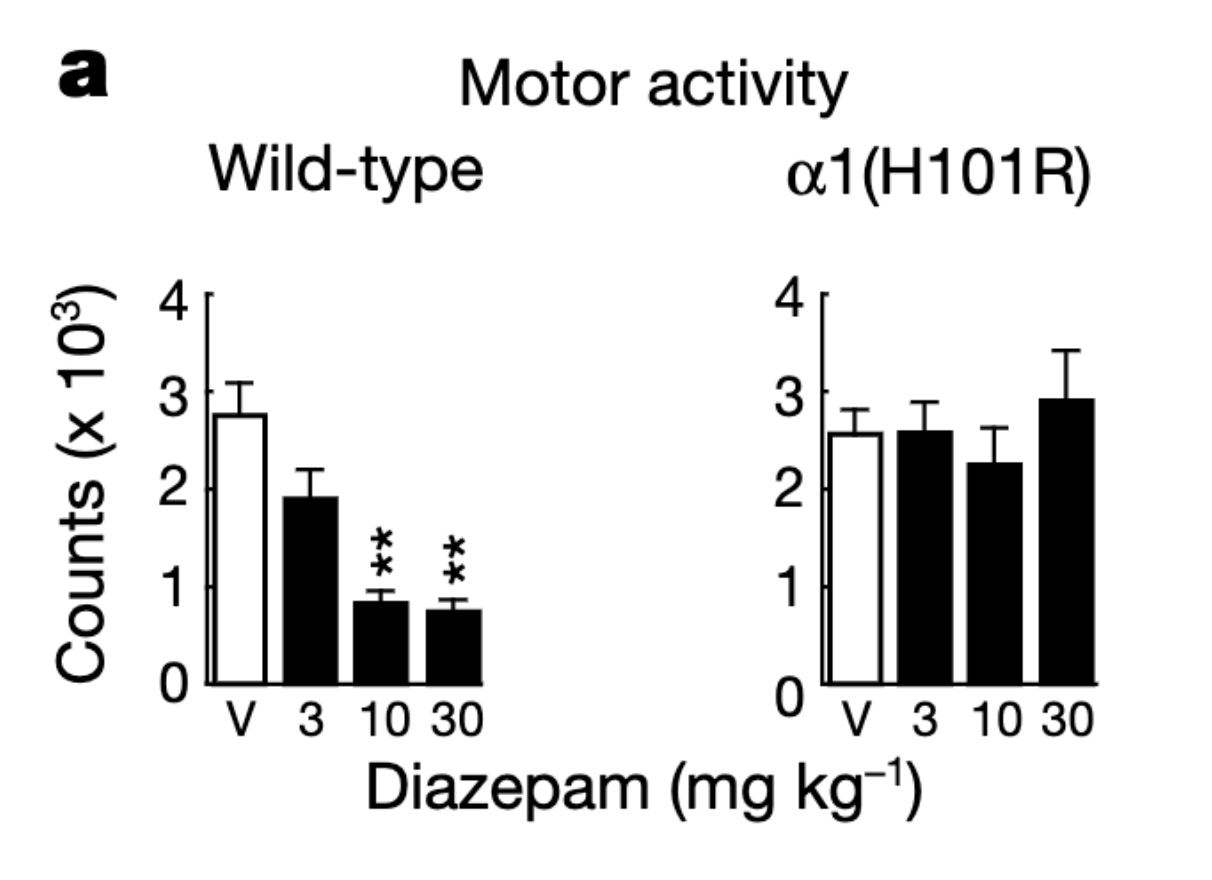
\includegraphics[width=.99\linewidth]{a1_sedation.png}
  \caption{Sedation test (measured in crossings of an enclosure)}
  \label{fig:test1}
\end{minipage}%
\begin{minipage}{.4\textwidth}
  \centering
  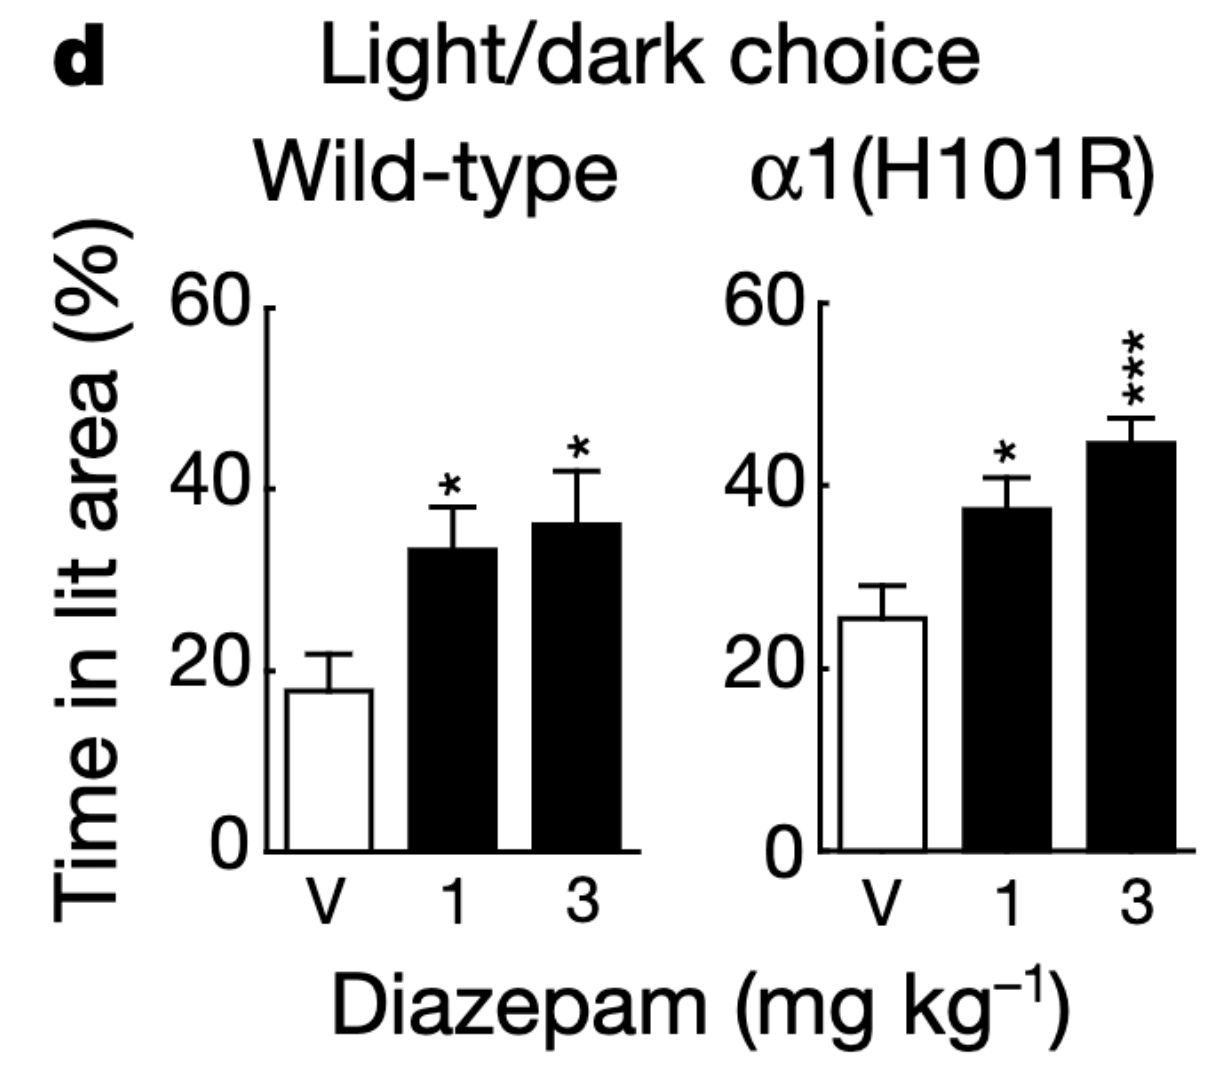
\includegraphics[width=.8\linewidth]{a1_anxiety.png}
  \caption{Anxiety test (measured in time spent in light areas (mice are typically scared of light open areas))}
  \label{fig:test2}
\end{minipage}
\end{figure}
\FloatBarrier

\textbf{Do these results suggest that a1 subunit containing GABA$_A$ receptors play a part in the sedative effects of benzodiazepines? Do these results suggest that a1 subunit containing GABA$_A$ receptors play a part in the anxiolytic effects of benzodiazepines?}

\section{}
Löw et al. repeated this experiment with the a2 and a3 subunits \cite{low_molecular_2000}. Their a2 results are shown in the figures below.

\FloatBarrier
\begin{figure}[H]
\centering
\begin{minipage}{.4\textwidth}
  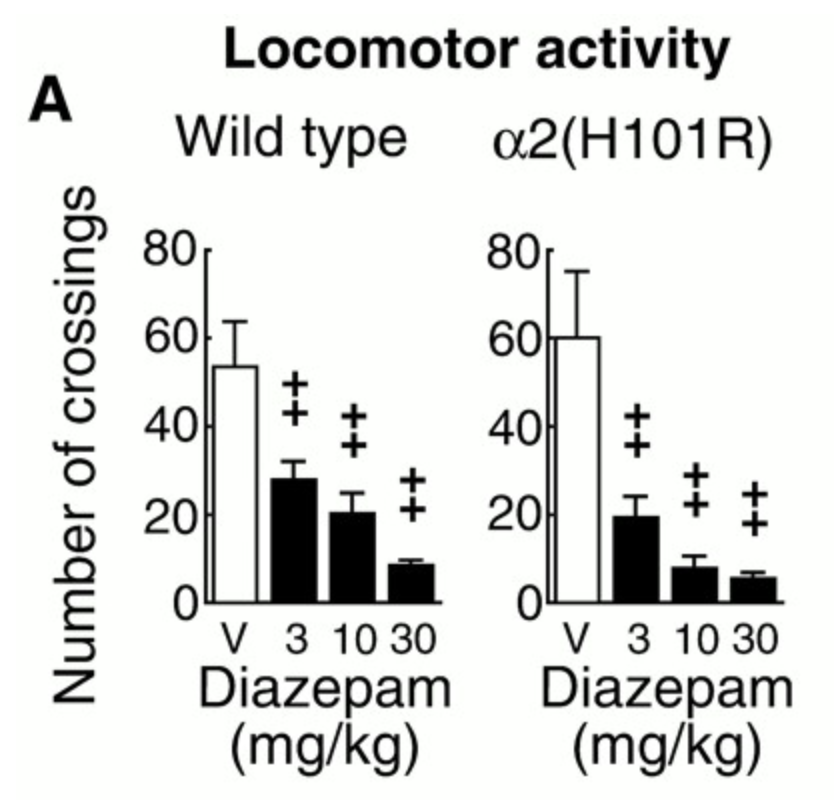
\includegraphics[width=.99\linewidth]{a2_sedation.png}
  \caption{Sedation test}
  \label{fig:test1}
\end{minipage}%
\begin{minipage}{.4\textwidth}
  \centering
  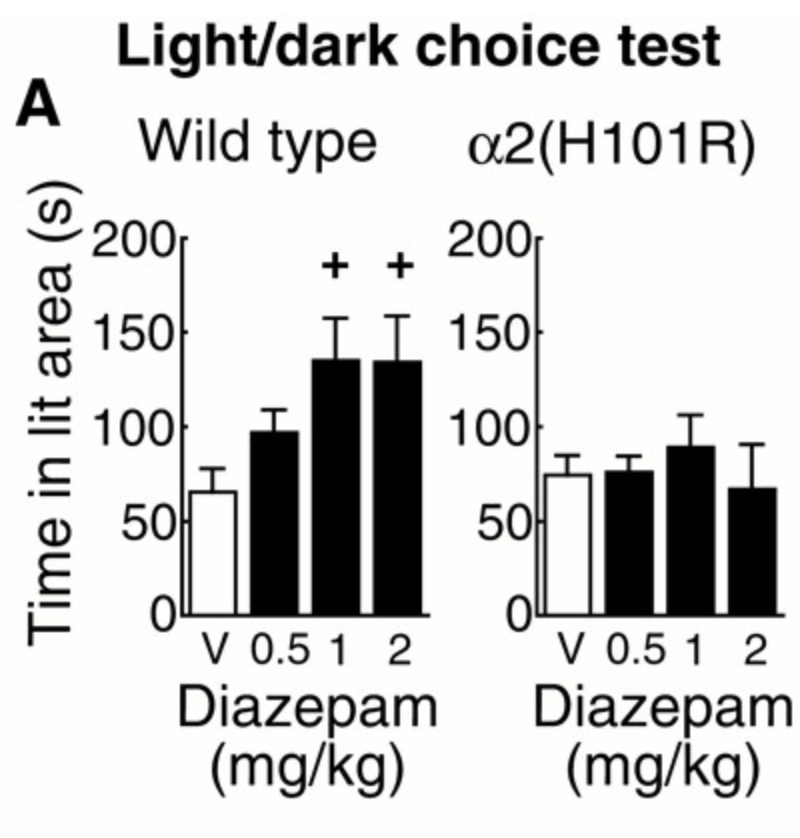
\includegraphics[width=.8\linewidth]{a2_anxiety.png}
  \caption{Anxiety test)}
  \label{fig:test2}
\end{minipage}
\end{figure}
\FloatBarrier
\textbf{Do these results suggest that a2 subunit containing GABA$_A$ receptors play a part in the sedative effects of benzodiazepines? Do these results suggest that a2 subunit containing GABA$_A$ receptors play a part in the anxiolytic effects of benzodiazepines?}

\section{}
Löw et al.'s a3 subunit results are shown in the figures below.

\FloatBarrier
\begin{figure}[H]
\centering
\begin{minipage}{.4\textwidth}
  \includegraphics[width=.99\linewidth]{a3_sedation.png}
  \caption{Sedation test}
  \label{fig:test1}
\end{minipage}%
\begin{minipage}{.4\textwidth}
  \centering
  \includegraphics[width=.8\linewidth]{a3_anxiety.png}
  \caption{Anxiety test)}
  \label{fig:test2}
\end{minipage}
\end{figure}
\FloatBarrier
\textbf{Do these results suggest that a3 subunit containing GABA$_A$ receptors play a part in the sedative effects of benzodiazepines? Do these results suggest that a3 subunit containing GABA$_A$ receptors play a part in the anxiolytic effects of benzodiazepines?}

\section{}
One of the brain regions that expresses the highest concentration of a2 containing GABA$_A$ receptors is the amygdala, which is known to be associated with fear responses. Does this observation align with the findings of the studies outlined in the previous questions?


\nocite{*}
\printbibliography
\end{document}
